\documentclass[a4paper]{article}

\usepackage{geometry}
\usepackage{natbib}
\bibpunct[:]{(}{)}{,}{a}{}{;}

%--------------------
%\usepackage{gb4e}
%\noautomath

\usepackage{amsmath}
\usepackage{amsfonts}
\usepackage{amsthm}
\usepackage{amssymb}
\usepackage{mathrsfs}
\usepackage{nicefrac}
%\usepackage{stmaryrd}
%\usepackage{multicol}
\usepackage{graphicx}
\usepackage{color}
%\newcommand{\mvalueof}[1]{\llbracket#1\rrbracket}
\newcommand{\citeposs}[2][]{\citeauthor{#2}'s (\citeyear[#1]{#2})}
\newcommand{\tuple}[1]{\ensuremath{\left\langle #1 \right\rangle}} 

\newcommand{\hl}[1]{\textcolor[rgb]{.8,.33,.0}{#1}}% prints in orange
%\newcommand{\argmax}[1]{\underset{#1}{\operatorname{arg}\,\operatorname{max}}\;}
%\newcommand{\argmin}[1]{\underset{#1}{\operatorname{arg}\,\operatorname{min}}\;}
%\newcommand{\sbna}{\exists\lnot\forall}

%--------------------
%
%\usepackage{setspace}
%\onehalfspacing
%
%-------------------


\title{Communicative pressures at the semantics-pragmatics interface:\\ Learning biases may prevent the lexicalization of pragmatic inferences}

\author{%\bf NAME1 and NAME2\\
    ( -- draft \today --- )
}


\date{}

\begin{document}
\maketitle

\begin{abstract} 
Mutual reasoning endows speakers with the ability to convey information that goes beyond the literal meaning of expressions. A particularity of certain classes of lexical meanings is that they enable for such pragmatic enrichments in a notably productive fashion. This raises the challenge to justify their regular selection over other alternatives that, e.g., do not require such enrichments. We suggest that such an account can be provided by an analysis of the linguistic pressures that apply at the semantics-pragmatics interface. To this end, we lay out a general model that combines functional pressure on language use and a pressure for learnability in acquisition in populations of probabilistic language users with varied degrees of pragmatic sophistication. We then use this model in a case study on the (lack of) lexicalization of scalar implicatures. The results suggest that such inferences fail to lexicalize when languages are pressured towards simpler semantic representations in learning, provided that pragmatic reasoning can compensate for the disadvantage in expressivity that users of such languages otherwise incur. We argue this result to shed light on the lack of lexicalization of scalar inferences, as well as the semantics-pragmatics distinction more generally.
\end{abstract}

\section{Introduction}\label{sec:introduction}
What is conveyed usually goes beyond what is said. A request for a blanket can be politely veiled by uttering ``I'm cold'', a temporal succession of events conveyed by the order in which conjunts appear, as in``I traveled to Paris and got married'', or an invitation be declined by saying ``I have to work''. An influential explanation of the relation between the literal meaning (semantics) of such expressions and what they are intended and interpreted to convey (pragmatics) sees the latter as a product of a process of mutual reasoning \citep{grice:1975}. For instance, under the assumption that the speaker is cooperative and strives to be relevant, ``I have to work'' may be interpreted as providing a reason why the speaker will not be able to accept the invitation -- why would she have said so otherwise?

Nowadays, it is common to draw a distinction between semantics and pragmatics in linguistic theorizing. Importantly, many classes of lexical meanings allow for pragmatic enrichments in a notably productive fashion. For instance, while John can eat all the cookies and still truthfully claim ``I ate some cookies'', the use of {\em some} over {\em all} is usually taken to convey that the latter does not hold. That is, ``I ate some cookies'' is pragmatically strengthened to convey that {\em some but not all} were eaten (\hl{citations for experimental evidence}). This inference is not restricted to quantifiers such as {\em some} and {\em all} but can be licensed for a large class of natural language expressions ranging from numerals such as {\em four} and {\em five} to adjectives such as {\em cold} and {\em big}.

These pragmatic inferences, so-called {\em scalar implicatures}, have been the focus of many theoretical and experimental studies at the semantics-pragmatics interface (\hl{citations}). However, an issue that has received little attention is the justification of semantic structure in light of the systematic enrichment offered by pragmatics. The present investigation seeks to fill this gap by analyzing the effects linguistic pressures have on the selection and pervasiveness of particular lexical meanings under consideration of their possible pragmatic enrichments.

\subsection{Linguistic pressures at the semantics-pragmatics interface}
The emergence and change of linguistic structure is influenced by many intertwined factors. These range from biological and socio-ecological to cultural \citep{steels:2011,tamariz+kirby:2016}. Social and ecological pressures determine communicative needs, while biology determines the architecture that enables and constrains the means by which they can be fulfilled. In the following, our focus lies on the remaining cultural aspect, wherein processes of linguistic change are viewed as shaped by language use and its transmission. That is, as a result of a process of cultural evolution. 

The idea that language is influenced by communicative pressures has played a pivotal role in synchronic and diachronic analyses at latest since \citeposs{zipf:1949} rationalization of the approximation of word frequency rankings by a power law distribution as competing hearer and speaker preferences (e.g. in \citealt{martinet:1962, horn:1984,jaeger+vRooij:2007,jaeger:2007, piantadosi:2014,kirby+etal:2015}). In recent years this line of research has led to a surge of approaches that seek to analyze the effects of such pressures on language from multiple angles ranging from simulations to experiments with human and robotic agents (see \citealt{steels:2015} and \citealt{tamariz+kirby:2016} for recent overviews). Our starting point is given by the overarching argument that has crystalized from the accumulated mathematical, experimental and cross-linguistic evidence in this literature: Natural languages need to be well-adapted to communicative needs within a linguistic community, but also need to be learnable to survive their faithful transmission across generations. More succinctly; natural languages are pressured for expressivity and learnability.   

The opposition of expressivity and learnability becomes particularly clear when considering their consequences in the extreme (cf. \citealt{kemp+regier:2012,kirby+etal:2015}). A language with a single form is easy to learn but lacking in expressivity. Conversely, a language that associates a distinct form with all possible meanings its users may want to convey is maximally expressive but challenging to acquire. The most prominent problem that arises from this tension is that of acquiring a language to express a potentially infinite set of meanings through finite means \citep{kirby:2002}. However, this is not the only challenge learners confront. A more central issue to our explanandum is that of selecting particular hypotheses out of a potentially infinite space of alternatives compatible with the data learners are exposed to. At the semantics-pragmatics interface this concerns the selection between functionally (near-)equivalent lexical meanings. Put differently, what is systematically conveyed through pragmatics could alternatively be codified lexically. However, lexical meanings that allow interlocutors to draw these inferences seem to resist their lexicalization. The question is why. We assume an integral part of the answer to be that learners are a priori biased towards simpler, more compressed, lexical representations. That is, rational learners should prefer simpler over more complex explanations of the data they witness \citep{feldman:2000, chater+vitanyi:2003, piantadosi+etal:2012a, kirby+etal:2015,piantadosi+etal:underreview}. In a nutshell, our hypothesis is that codifying more semantically is a priori dispreferred by learners. Crucially, in cases where pragmatics offers conventional means of enrichment, the communicative disadvantage that speakers would otherwise incurr is leveled. In this way, semantics and pragmatics play a synergic role in overcoming linguistic pressures for expressivity and learnability which may prevent the lexicalization of pragmatic inferences.  

In the following, we model these components using the replicator-mutator dynamics, combining functional pressure on successful communication with effects of learning biases on (iterated) Bayesian learning \citep{griffiths+kalish:2007}. The semantics-pragmatics distinction and its effect on production and comprehension are captured by a probabilistic model of rational language use with different degrees of pragmatic sophisitication and languages \citep{frank+goodman:2012,franke+jaeger:2014, bergen+etal:2016}. The remainder of this section introduces these components individually together with the assumptions underlying them. These are: the representation of languages and their use (\S\ref{sec:languages+use}), pressures towards expressivity (\S\ref{sec:expressivity}) and learnability (\S\ref{sec:learnability}), regulated by the replicator and mutator dynamics, respectively, as well as a bias towards simpler semantic representations, codified as the learners' prior. After laying out the model, we analyze its predictions in a case-study on the lack of lexicalization of scalar implicatures in \S\ref{sec:si-case-study}.  



\subsection{Lexica and linguistic behavior}\label{sec:languages+use}
Lexica codify the truth-conditions of a language's expressions, i.e., its semantics. Following e.g. \citet{franke+jaeger:2014}, a convenient way to represent lexica is by $(|S|,|M|)$-Boolean matrices, where $S$ is a set of states of affairs (meanings) to convey and $M$ a set of messages (forms available in the language). For example, the following two fragments determine the truth-conditions of two messages, $m_1$ and $m_2$, for two states, $s_1$ and $s_2$.

\begin{centering}
$L_a$ = \bordermatrix{~ & m_1 & m_2 \cr 
                  s_1 & 1 & 0 \cr
                  s_2 & 1 & 1 \cr} \hspace{2cm} $L_b$ = \bordermatrix{~ & m_1 & m_2 \cr 
                  s_1 & 1 & 0 \cr
                  s_2 & 0 & 1 \cr}\\[0.5cm]
\end{centering}


According to lexicon $L_a$ the message $m_1$ is true of state $s_1$ as well as of $s_2$. In contrast, $m_1$ is only true of $s_1$ in $L_b$. Otherwise, the two languages are truth-conditionally equivalent. 

While these representations are very coarse and simple, they suffice to make the distinction between semantics and pragmatics precise. We distinguish between two kinds of linguistic behavior. {\em Literal interlocutors} produce and interpret messages literally. That is, their linguistic choices are guided only by their lexica. In contrast, {\em pragmatic interlocutors} engage in mutual reasoning to inform their choices. For instance, a rational speaker of $L_a$ who reasons about her addressee may use $m_1$ to exclusively signal state $s_1$ since $s_2$ can unambiguously be conveyed through $m_2$. Accordingly, rational hearers that expect their interlocutor to reason along these lines will interpret ambiguous $m_1$ as $s_1$. An important consequence of this process of mutual reasoning for our purposes is that it can render $L_a$ (nearly) indistinguishable from $L_b$ in terms of language use.

Following models of rational language use such as Rational Speech Act models \citep{frank+goodman:2012} and their game-theoretic predecessors, the Iterated Best/Quantal Response models \citep{franke:2009,franke+jaeger:2014}, this kind of signaling behavior is captured by a reasoning hierarchy. The hierarchy's bottom, level $0$, corresponds to literal language use. Pragmatic language users of level $n + 1$ behave rationally according to expected level $n$ behavior of their interlocutors. Below, (\ref{h:level0}) and (\ref{h:leveln}) specify the behavior of literal and pragmatic hearers of a language $L$. Literal and pragmatic speakers are specified in (\ref{s:level0}) and (\ref{s:leveln}).

\begin{flalign}
&H_{0}(s|m;L) \propto pr(s) L_{sm} \label{h:level0}\\
&S_{0}(m|s;L) \propto \exp(\lambda \; L_{sm}) \label{s:level0}\\
&H_{n+1}(s|m;L) \propto pr(s) S_{n}(m|s;L) \label{h:leveln}\\
&S_{n+1}(m|s;L) \propto  \exp(\lambda \; H_{n}(s|m;L)^\alpha) \label{s:leveln}
\end{flalign}

According to (\ref{h:level0}), a literal hearer's interpretation of a message $m$ as a state $s$ depends on her lexicon and her prior over states, $pr \in \Delta(S)$. In the following this prior is assumed to be uniform across hearers. The behavior of literal speakers, given in (\ref{s:level0}), is regulated by a soft-max parameter $\lambda$, $\lambda \geq 1$ \citep{luce:1959,sutton+barto:1998}. As $\lambda$ increases, choices made in production are more rational in that higher values lead to behavior that is increasingly in line with expected utility maximization. 

Pragmatic behavior is similar to its literal counterparts. As hinted at in the informal sketch above, their difference lies in that level $n+1$ speakers/hearers reason about level $n$ hearer/speaker behavior instead of solely relaying on their lexicon. That is, they reason about the way a rational level $n$ interlocutor would use or interpret a message, and behave according to these expectations. Pragmatic production is further regulated by a parameter $\alpha$ which controls the tension between semantics and pragmatics, $\alpha \in (0,1]$. Lower values lead to more literal production whereas higher values lead to stronger pragmatic behavior. 

We call the combination of a lexicon with its use, i.e., a level in the reasoning hierarchy, a type. These are the basic units on which our population dynamics operate. 

\subsection{Replication \& expressivity}\label{sec:expressivity}
Expressivity has received particular attention from investigations using evolutionary game theory (e.g. \citealt{nowak+krakauer:1999,nowak+etal:2000, nowak+etal:2002}). Under this view, a type's ability to convey and interpret information successfully confers it a higher fitness, a measure that is relative to the success of other types in the population. In the simplest models fitness directly translates into the proportion of types present in the population after a generational turnover. As a consequence, fitter types flourish while unfit ones are driven out. This association of communicative success within a population with changes in the proportion of types present in it creates a feedback loop that pressures the population towards greater expressivity. 

The replicator equation gives us the means to make these dynamics precise. The proportion of types in a given population is codified in a vector $x$, where $x_i$ is type $i$'s proportion. As noted above, the fitness of type $i$ is equal to its relative communicative success within this population, $f_i = \sum_j x_j \text{EU}(t_i,t_j)$. That is, its fitness is the sum of its expected communicative success in interacting with other types weighted by the latter's population share. Communicating well with types that appear often thusly confers a higher fitness than doing so with underrepresented ones. The expected communicative success of $i$ and $j$ is obtained by considering the average success of $i$ conveying information to $j$ and vice versa: $\text{EU}(t_i,t_j) = [U_S(t_i,t_j) + U_R(t_i,t_j)]/2$. $U_S(x,y)$ and $U_R(x,y)$ are, respectively, $\sum_s P(s)\sum_m S_n(m|s;L) \sum_{s'} R_o(s'|m;L) \delta(s,s')$ and $U_S(y,x)$, for $n$ and $o$ being the reasoning level of $x$ and $y$, and $\delta(s,s') = 1$ iff $s = s'$ and $0$ otherwise. This quantity is symmetric, reflecting the probability of two types' mutual understanding. The average fitness of the population is given by $\Phi$, $\Phi = \sum_i x_i f_i$. This term serves as a normalizing constant for the discrete replicator equation: $\dot{x}_i = \frac{x_i f_i}{\Phi}$ 

Under its biological interpretation, this equation captures the idea of fitness-relative selection whereby fitter types produce more offspring, leading to their propagation in subsequent generations. As noted in \S\ref{sec:introduction}, many aspects of language are subject to processees of transmission and change that can be likened to these biological dynamics. Amongst others, replication can be construed as modelling language acquisition, as e.g. in \citealt{nowak+etal:2002}, but also as a process of horizontal adaptation in a single generation (see \citealt[\S3.3]{benz+etal:2005b} for discussion).

In their series of papers on language evolution, Nowak and colleagues did not only consider expressivity but also recognized the central role played by the fidelity by which languages are transmitted. Linguistic production can be prone to errors and multiple languages may be compatible with the data learners are exposed to. These sources of uncertainty introduce variation in their faithful acquistion. In keeping the analogy to evolutionary processes this variation can be likened to mutation to the effect that a type's offspring may adopt a different type than that of its parent. Importantly, the resulting generational turnovers should depend on the relative learnability of a type. For this purpose, we turn to a different strand of research in cultural evolution: {\em iterated learning}. 

%errors were considered in N+K:1999, mutation in N+etal:2002

\subsection{Mutation \& learning}\label{sec:learnability}
Iterated learning is a process in which the behavior of one individual serves as learning input for another. This learner, upon acquisition of this behavior, then goes on to produce behavior that serves as input for a new learner. This process can be thought of as a progression through chains of parents and children; the parent produces linguistic data from which the child infers a language. The latter, now a parent, goes on to produce linguistic data for a new generation of na\"ive learners. Following \citet{griffiths+kalish:2007} we model iterated learning as a repeated process of Bayesian inference in which learners combine the likelihood of a type producing the received learning input with prior inductive biases. 



Due to the pressure towards learnability it exherts, iterated learning generally leads to simpler and more regular languages (see \citealt{kirby+etal:2014} and \citealt{tamariz+kirby:2016} for recent surveys). Importantly, experimental and mathematical results suggest that the outcome of this process reflects learners' a priori biases. In a Bayesian setting these biases can be codified in a prior $P \in \Delta(T)$. A way to think about this prior is as the amount of data a learner would require in order to adopt a language (cf. \citealt[450]{griffiths+kalish:2007}). Or, in our case, a combination of a lexicon and a signaling behavior. 

As touched upon in \S\ref{sec:introduction} we assume learners to be biased towards simpler semantics. That is, learners have a preference for types that can explain the data by codifying less in their lexical representations. More generally, a drive for simplicity has been argued to underpin speaker preferences for brevity and ease of articulation, as well as to pressure languages towards lexical ambiguity and grammatical compression \citep{zipf:1949,grice:1975,piantadosi+etal:2012, kirby+etal:2015}. As shown by \citet{chater+vitanyi:2003} simplicity not only provides a solution to problems of induction by allowing for the distinction between equally explanatory hypotheses, but it has also proven its empirical worth as a predictive principle in cognitive modelling.  

The extent of the prior's influence has been shown to heavily depend on the learning strategy assumed to underly the inference process. On the one hand, simulation results suggested that weak biases could be magnified by exposing learners to only small data samples \citep{brighton:2002}. On the other, \citeposs{griffiths+kalish:2007} mathematical characterization showed that iterated learning converged to the prior. That is, the distribution over languages obtained from this process corresponded to the learners' prior distribution and was independent of the amount of input given to them. This difference in predictions can be traced back to differences in the selection of hypotheses from the posterior. Griffith \& Kalish's convergence to the prior holds for learners that sample from the posterior. More deterministic strategies such as the choice for the type with the highest posterior probability, so-called {\it maximum a posterior estimation} (MAP), increase the influence of both the prior and the data \citep{griffiths+kalish:2007,kirby+etal:2007}. In the following, we parametrize the posterior by $l \geq 1$. In doing so, we obtain a range of learning strategies that live between posterior sampling and MAP. When $l = 1$ learners sample from the posterior. As $l$ increases towards infinity their propensity to maximize the posterior grows as well. 

The data learners are exposed to is described by a set $D$ containing sequences of state-message pairs, e.g., $\tuple{\tuple{s_i,m_v},...\tuple{s_j,m_w}}$. These correspond to sequences of of language use witnessed by the learners. In the following, we denote the length of these sequences by $k$. Put differently, each datum $d \in D$ contains $k$ members of the set $\{\tuple{s_i,m_v} | s_i \in S, m_v \in M\}$.

To summarize, the parametrized posterior, $P(d|t)^l$, is obtained from combining the prior $P(t)$ and the likelihood $P(d|t)$. Since types are combinations of a lexicon and its use, the latter can be computed straightforwardly from the type's production. We combine the replicator dynamics with iterated learning by codifying these components in a transition matrix $Q$. $Q_{ij}$ indicates the probability that a child of a parent of type $i$ adopts type $j$. This quantity is proportional to the probability of $i$ producing the learning data and that of inferring $j$ given the data: 

\[
 Q_{ij} \propto \sum_{d \in D} P(d|t_i) F(t_j,d),
\]
where $F(t_j,d) \propto P(t_j|d)^l$ and $P(t_j|d) \propto P(t_j) P(d|t_j)$.
 

\subsection{Summary}
Drawing from past research, we argued that expressivity, learnability and simplicity are central to the cultural evolution of language. In the present setup they are modelled as communicative efficiency-relative replication, iterated Bayesian learning, and a prior that biases learners for compressed lexical meanings. Taken together their dynamics are described by the replicator-mutator dynamics \citep{hofbauer+sigmund:2003}: 

\[ 
\hat{x}_i = \sum_j Q_{ji} \frac{x_jf_j}{\Phi}
\]

The units that the dynamics operate on are a combination of a lexicon and a degree of pragmatic sophistication which determines its use. We call this combination a type. A type's expressivity depends on its communicative efficiency within a population while its learnability depends on the fidelity by which it is infered by new generations of na\"ive learners. With this model at hand we turn to the analysis of the lack of lexicalization of productive pragmatic inferences.

\section{Scalar implicatures}\label{sec:si-case-study}
%
Scalar implicatures are a particularly well-studied type of conventional pragmatic inference. They are licensed for groups of expressions ordered in terms of informativity, here understood as an entailment induced order. For instance, {\em some} is entailed by {\em all}. If it were true that `All students came to class', it would also be true that `Some students came to class'. However, as already noted in \S\ref{sec:introduction}, while weaker expressions such as {\em some} are truth-conditionally compatible with stronger alternatives such as {\em all}, this is not what their use is normally taken to convey. Instead, the use of a less informative expression when a more informative one could have been used can license a defeasible inference that stronger alternatives do not hold (cf. \citealt{horn:1972,gazdar:1979}). That is, a hearer who assumes the speaker to be able and willing to provide all relevant information can infer that stronger alternatives do not hold since the speaker did not use them. In this way, `Some students came to class' is strengthened to convey that some but not all students came to class. Conversely, speakers can rely on their interlocutors to draw this inference. The bound that rules out stronger alternatives is thusly not codified in the lexical meaning of weak alternatives but instead pragmatically supplied.

This kind of strengthening corresponds to our previous description of the pragmatic use of lexicon $L_a$. A pragmatic hearer who reasons about a speaker's use of message $m_1$ will associate it more strongly with $s_1$ than with $s_2$ since the latter is already unambiguously associated with $s_2$. Conversely, a pragmatic speaker will reason about her interlocutor's interpretation and use the messages accordingly. 

\begin{centering}
$L_a$ = \bordermatrix{~ & m_1 & m_2 \cr 
                  s_1 & 1 & 0 \cr
                  s_2 & 1 & 1 \cr} \hspace{2cm} $L_b$ = \bordermatrix{~ & m_1 & m_2 \cr 
                  s_1 & 1 & 0 \cr
                  s_2 & 0 & 1 \cr}\\[0.5cm]
\end{centering}

Our initial question can now be narrowed in terms of scalar implicatures by asking for a justification for the lack of lexical upper-bounds in weak scalar alternatives. That is, why semantics such as those of message $m_1$ in $L_a$ are regularly selected for over the alternative of codifying the bound semantically as in $L_b$. More poignantly, would it not serve language users better if weak(er) expressions such as {\em warm}, {\em or}, {\em some} and {\em big} were truth-conditionally incompatible with stronger alternatives such as {\em hot}, {\em and}, {\em all} and {\em huge}?  This question is particularly striking considering the number of expressions suggested to license such inferences across languages. 

We see two main explanations for the lack of upper-bounds in the lexical meaning of weak scalar expressions. The first is that their truth-conditional compatibility with stronger expressions endows them with a broader range of applicability by allowing them to occur in contexts in which their upper-bounded reading is absent. This can happen when embedded in downward-entailing contexts, when the speaker is likely uncertain about whether the upper bounded reading is true, or when the distinction between an upper-bounded reading and the simple, only lower-bounded reading, is not relevant. For instance, if for all the speaker knows `Some students came' but she doesn't know whether all came, then the use of unbounded {\em some} succinctly conveys her uncertainty. This may suggest a functionalist argument for why upper-bounded meanings do not conventionalize: should contextual cues provide enough information to the hearer to identify whether a bound is intended to be conveyed pragmatically, then this is preferred over expressing it overtly through longer expressions. For example, by saying {\em some but not all} explicitly. Importantly, although morphosyntactic disambiguation is dispreferred due to its relative length and complexity, it allows speakers to enforce an upper-bound and override contextual cues that might otherwise mislead the hearer. In a nutshell, this explanation posits that scalar implicatures fail to lexicalize because, all else being equal, speakers prefer to communicate as economically as possible and pragmatic reasoning enables them to do so. Compare this with a hypothetical language that lexicalizes two expressions for each weak scalar expression -- one with and one lacking an upper-bound. Along this functionalist explanation, we see four conditions that may pressure languages for English-like semantics over this alternative. First, contextual cues are very reliable. Second, morphosyntactic disambiguation is seldom necessary. Third, morphosyntactic disambiguation is only marginally dispreferred. Fourth, larger lexica are costly. Overall, neither condition is convincing as a pivotal explanatory device for such a wide-spread phenomenon. The first two conditions put a heavy burden on the ability to retrieve contextual cues to a degree that seems unlikely to undercut the benefit of unambiguous communication. It is likely that human language users are very good at retrieving cues from context, but to stipulate that they are so good as to undercut the benefit of safe communication provided by our hypothetical alternative strikes us as too strong of an assumption.  As for the third and fourth condition, these seem mostly like technical solutions without a proper empirical basis. 

Taking the regularity and spread of scalar implicatures together with the observation that monomorphemic expressions that lexically rule out stronger alternatives are unattested across languages (\citealt[252-267]{horn:1984},\citealt{horn:1972,traugott:2004,vdAuwera:2010}) suggests that other forces may be play. In what follows we investigate the hypothesis that the lack of lexicalization of scalar inferences can be accounted for through the relative simplicity of lexical meanings lacking an upper-bound over those that explicitly codify it. While we do not want to argue that functionalist pressure may not play a role, we do see a clear benefit in exploring whether matters of learnability would not give us additional leverage.


Note however that we do not represent the contrast between lexical representations explicitly. Instead, the learning bias towards a lack of upper-bounds in weak scalar alternatives is directly encoded in the learners' prior over types. In principle this difference could be made precise with an adequate representational language, e.g., through measures over representational complexity such as minimal description length.  There is a growing effort to develop such empirically  testable  representational  languages. For  instance, the so-called language of thought has been put to test in various rational probabilistic models that show encouraging results (see e.g. \citealt{katz+etal:2008, piantadosi+etal:underreview, piantadosi+etal:2012} and references therein). We think that our assumption is well-warranted as a working hypothesis and decide against such an enrichment given that the introduction of a larger framework would also require further assumptions and justifications. 
 

\subsection{Analysis}
We analyze the model's predictions in populations of types with two signaling behaviors; literal or pragmatic. The former correspond to level $0$ reasoners who only take their lexica into consideration and the latter to level $1$ reasoners. Higher level reasoning is not required to derive scalar implicatures from the lexica we consider here nor would it provide substantial pragmatic refinement.

The space of possible lexica is given in Table \ref{tab:lexica}. As in the preceding examples, lexica are $(2,2)$-Boolean matrices. These are the simplest matrices that allow us to make the contrast between the presence or lack of an upper-bound and the use of scalar implicatures precise. As implicit in the discussion so far, one may think of $s_1$ as a ``some but not all''-state and of $s_2$ as an ``all''-state. The literal meaning of weak scalar expressions such as English {\em some} then corresponds to a message true of both $s_1$ and $s_2$ in these fragments. Following our assumption for a preference for simple lexical representations, the prior biases learners against lexica in which a message holds true only of state $s_1$. That is, those messages that lexicalize an upper-bound that rules out the ``all''-state $s_2$. All other semantics are assumed to be a priori equally probable. Accordingly, this prior is captured by $P(t_i) \propto n - c \cdot r$, where $n$ is the total number of states and $r$ is the number of messages only true of $s_1$ in $t_i$'s lexicon, $c \in [0,1]$. In short, increments in parameter $c$ bring about a stronger preference against languages that lexicalize upper-bounds, i.e., $L_2, L_4$ and $L_6$.

\begin{table}[t]
\centering 
\begin{tabular}{l c l}
$L_1$ = $\begin{pmatrix} 0 & 0 \\ 1 & 1 \end{pmatrix}$ & 
$L_2$ = $\begin{pmatrix} 1 & 1 \\ 0 & 0 \end{pmatrix}$ & 
$L_3$ = $\begin{pmatrix} 1 & 1 \\ 1 & 1 \end{pmatrix}$\\[0.5cm]

$L_4$ = $\begin{pmatrix} 1 & 0 \\ 0 & 1 \end{pmatrix}$ &
$L_5$ = $\begin{pmatrix} 1 & 0 \\ 1 & 1 \end{pmatrix}$ &
$L_6$ = $\begin{pmatrix} 1 & 1 \\ 0 & 1 \end{pmatrix}$
\end{tabular}
\caption{Space of possible lexica.}
\label{tab:lexica}
\end{table}


While there is a total of $16$ possible $(2,2)$-lexica, a number of them are identical both in terms of expressivity and the learning bias. The competition between such types is determined by the initial configuration of a population, i.e., the proportion with which each type starts out. However, this fact can be obscured when averaging across simulations. We therefore focus on a smaller representative subset.\footnote{Simulations conducted with the full space of possible lexica confirm that the results reported here do not hinge on their exclusion.} Lexica $L_1$ to $L_3$ are not optimal for communication because they assign the same state to all their messages. This failure to associate a single form to a meaning both semantically and pragmatically inevitably leads to their disadvantage in language use. $L_4$ and $L_5$ are our target lexica, previously labeled as lexica $L_b$ and $L_a$. They codify upper-bounded semantics for message $m_1$ and a lack thereof, respectively. Lastly, $L_6$ is similar to $L_5$ in that two messages are true of the same state but differs from it in assigning upper-bounded semantics to $m_1$. 


Combining a signaling behavior with each of these $6$ lexica yields a total of $12$ distinct types. Note in particular  that a type that has conventionalized upper bounds to realize a (quasi-)partition of the relevant semantic space, such as $L_4$, will produce speaker behavior that is {\em almost} indistinguishable from that of a language that lacks upper bounds, but with pragmatic speakers, such as $L_5$. Almost, because there may be slight differences between the probability with which speakers would (erroneously) use a semantically false description and the probability with which speakers would (erroneously) use a pragmatically suboptimal description. Due to this possibly marginal difference between pragmatic $L_4$ and $L_5$, the selection of one type over the other is expected to mainly depend on the learning bias. Things are less clear for literal $L_5$ contrasted with literal/pragmatic $L_4$. The former has a learning advantage but is expected to fare worse in communicative  terms in virtue of ambiguous $m_1$.


The dynamics are initialized with an arbitrary distribution over types, constituting the population's first generation. The results for each parameter setting were obtained from $1000$ independent runs, each consisting of $20$ generations. This corresponds to a developmental plateau after which no noteworthy change was registered. As specified in \S\ref{sec:learnability}, the learning matrix $Q$ can be obtained by considering all possible state-message sequences of length $k$. Given that this is intractable for large $k$, matrices were approximated by sampling $10$ sequences from each type's production probabilities and a type's children being exposed only to this subset. For convenience, the model's parameters are summarized in Table \ref{tab:summary}.

\begin{table}
\centering
\begin{tabular}{l|l|l}
    \multicolumn{1}{c}{parameter} & \multicolumn{1}{c}{explanation} & \multicolumn{1}{c}{locus}\\ \hline
    $\lambda \geq 1$ & rationality parameter & $S_{n+1}(m|s;L) \propto \text{exp}(\lambda \; H_{n}(s|m;L)^\alpha)$\\
    $\alpha \in [0,1)$ & semantics-pragmatics tension & $S_{n+1}(m|s;L) \propto \text{exp}(\lambda \; H_{n}(s|m;L)^\alpha)$\\ 
    $|D|$ & number of data produced per parent type & $P(d|t_j)P(t_i|d)$\\
    $k = |d|$ & number of observations per datum& $P(d|t_j)P(t_i|d)$\\
    $l \geq 1$ & posterior parameter from sampling to MAP & $P(t_i|d) \propto [P(t_i)P(d|t_i)]^l$\\
    $c \in [0,1]$ & learning bias for lack of upper-bounds &  $P(t_i)$
\end{tabular}
\caption{Summary of model parameters.} 
\label{tab:summary}
\end{table}

According to our hypothesis, functional pressure on successful communication combined with learning pressures in the form of a bias against upper-bounds may lead to the selection of $L_5$-like semantics. It is instructive to first inspect the effect of these pressures in isolation. For this purpose we focus our attention on three pragmatic types.\footnote{Pragmatic reasoning allows language users to refine their (possibly erroneous) choices. Therefore, it is advantageous even for those types that codify an upper-bound lexically.} Pragmatic $L_3$, a type that is lacking in expressivity but is a priori preferred for its lack of upper-bounds. Pragmatic $L_4$, a type that is functionally advantageous but biased against. And pragmatic $L_5$, combining virtues of the latter two.  

\paragraph{Expressivity only.} Recall that the replicator dynamics are sensitive to $\lambda$ and $\alpha$ as both have a bearing on a type's fitness. In particular, low $\alpha$ disadvantages types that rely on pragmatic reasoning to the gain of those that codify more semantically. The rationality parameter $\lambda$ has a similar effect for different reasons: Low rationality leads to a less pronounced preference for the choice(s) expected to succeed best in communication. That is, $\lambda$ regulates the strength by which users of $L_5$ associate non-upper-bounded $m_1$ exclusively with the ``some''-state $s_1$ over the ``all''-state $s_2$. Speakers of $L_4$ need not rely on $\lambda$ for this, as as the association of $m_1$ with $s_1$ is already part of their language's semantics.

The effect of the rationality parameter for $\alpha = 1$ is depicted in Figure \ref{fig:either-R-or-M}.A. As expected, the less expressive $L_3$ speakers fare the worse and are influenced the least by variations in $\lambda$. In contrast, low values of $\lambda$ result in a higher proportion of $L_4$ speakers relative to $L_5$. This is expected given role of rationality in producing more deterministic linguistic behavior in users of $L_5$-like languages. As the rationality parameter increases the functional difference between $L_4$ and $L_5$ is levelled. Overall, the final populations that result only from a pressure towards expressively come close to an even share of pragmatic $L_4, L_5$ and $L_6$ types (the latter follows the same trajectory as $L_5$ in Figure \ref{fig:either-R-or-M}).  That is, expressivity alone can not differentiate between these lexica in populations of rational pragmatic language users.  

\begin{figure}
\centering
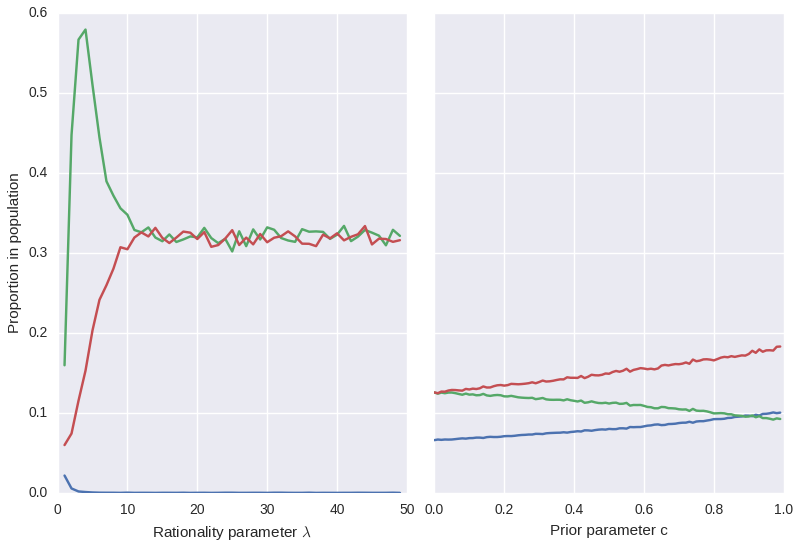
\includegraphics[scale=.5]{./only-R-or-M}
\caption{Mean proportions of target types after $20$ generations in $1000$ populations with only replication (A; $\alpha = 1$) and only mutation (B; $\alpha =1, \lambda = 30, k = 5$).}
\label{fig:either-R-or-M}
\end{figure}

\paragraph{Learnability only.} The effect of iterated learning without a pressure for expressivity is shown in Figure \ref{fig:either-R-or-M}.B with posterior sampling. In line with our expectations, the share of $L_4$ speakers decreases as the bias against this lexicon increases. In turn, this benefits $L_3$ and, in particular, $L_4$. However, note that even a strong bias against lexical upper-bounds leads only to a moderate advanage for $L_5$ over $L_4$. Furthermore, a pressure only towards learnability can promote functionally defective languages $L_3$.

Inspecting these pressures separately not only gives some intuitions about the parameters' influence, but also highlights some of their broader implications. First and foremost, neither dynamic comes close to converging to a monomorphic population under most parameter configurations. For instance, while $L_4$ speakers can come to take over a substantial proportion of the population, this only happens in a restricted range of low degrees of rationality. Apart from polymorphy, both pressures make undesirable predictions. A pressure only towards expressivity leads to the selection of types using $L_4$ to $L_6$ and to the ejection of $L_1$ to $L_3$. However, it can not explain the regular selection of $L_5$-like semantics over either of these functionally similar alternatives. In contrast, a pressure only towards learnability has a modest but clear effect in differentiating $L_5$ from these alternatives but fails to rule out functionally suboptimal types such as tautological $L_3$. In sum, neither dynamic on its own is a suitable candidate to provide a justification for the predicted prevalence of $L_5$-like semantics. 

\begin{figure}
\centering
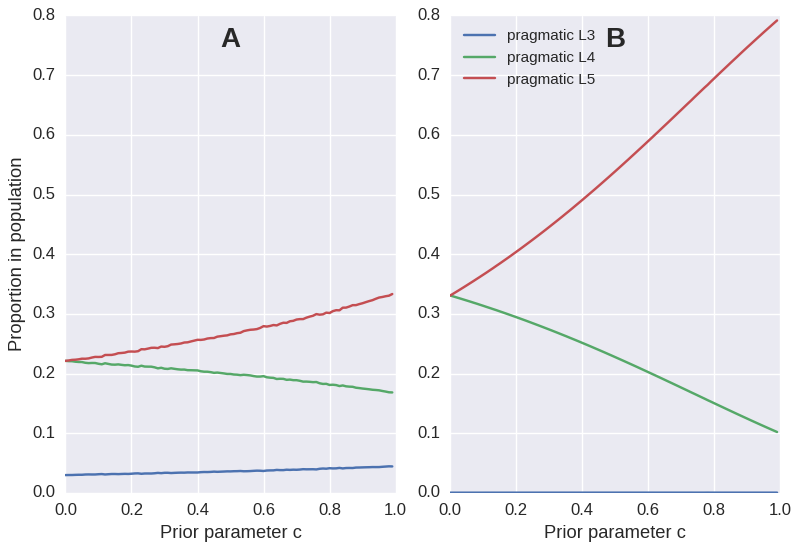
\includegraphics[scale=.5]{./fig2-rmd}
\caption{Mean proportions of target types after $20$ generations in $1000$ populations across bias values $c \in [0,1]$ with $l =1$ in A and $l = 3$ in B ($\alpha =1, \lambda = 20, k = 5$).}
\label{fig:cost}
\end{figure}

\paragraph{Expressivity and learnability.} Figure \ref{fig:cost} illustrates the effect of the learning bias for posterior sampling (\ref{fig:cost}.A) and slightly more MAP-like learning (\ref{fig:cost}.B). More detailed results for all types across a sample of $c$-values are presented in Table \ref{tab:numeric-results}. Overall, these results suggest that in the present setup a weak bias is sufficient to lead to a selection of $L_5$ over $L_4$. As in the simulations that only considered learnability, this effect increases with the bias' strength provided $L_5$ users are pragmatic. Importantly, the addition of a pressure towards expressivity magnifies this effect and dampens the proliferation of functionally suboptimal types advantaged by the learning bias. As stressed above, this suggests that neither the learning bias nor functional pressure alone but their combination may lead to the lack of upper-bounds in the lexical meaning of scalar expressions.


\begin{table}
\centering 
\begin{tabular}{l | c c c c c| c c c c c c c c}
\multicolumn{1}{c}{~} & \multicolumn{5}{c}{$l = 1$} & ~ & \multicolumn{5}{c}{$l = 3$}\\ \hline \hline
  c        &  0  & .1  & .5  & .8  & .9 & ~ & 0 & .1 & .5 & .8 & .9\\ \hline \hline
lit. $L_1$ & .03 & .03 & .04 & .04 & .04& ~ & $\epsilon$ & $\epsilon$ & $\epsilon$ & $\epsilon$ & $\epsilon$\\ 
lit. $L_2$ & .03 & .03 & .02 & .01 & .04& ~ & $\epsilon$& $\epsilon$ & $\epsilon$ & $\epsilon$ & $\epsilon$\\
lit. $L_3$ & .03 & .03 & .04 & .04 & .04& ~ & $\epsilon$& $\epsilon$ & $\epsilon$ & $\epsilon$ & $\epsilon$\\
lit. $L_4$ & .07 & .07 & .06 & .06 & .05& ~ & $\epsilon$& $\epsilon$ & $\epsilon$ & $\epsilon$ & $\epsilon$\\
lit. $L_5$ & .04 & .05 & .05 & .06 & .06& ~ & $\epsilon$& $\epsilon$ & $\epsilon$ & $\epsilon$ & $\epsilon$\\
lit. $L_6$ & .04 & .04 & .04 & .04 & .03& ~ & $\epsilon$& $\epsilon$ & $\epsilon$ & $\epsilon$ & $\epsilon$\\ \hline
prg. $L_1$ & .03 & .03 & .04 & .04 & .04& ~ & $\epsilon$& $\epsilon$ & $\epsilon$ & $\epsilon$ & $\epsilon$ \\
prg. $L_2$ & .03 & .03 & .02 & .01 & .04& ~ & $\epsilon$& $\epsilon$ & $\epsilon$ & $\epsilon$ & $\epsilon$ \\
prg. $L_3$ & .03 & .03 & .04 & .04 & .04& ~ & $\epsilon$& $\epsilon$ & $\epsilon$ & $\epsilon$ & $\epsilon$ \\ 
prg. $L_4$ & .22 & .22 & .2 & .18 & .17& ~ & .33& .31 & .23 & .15 & .12 \\
prg. $L_5$ & .22 & .23 & .27 & .3  & .32& ~ & .33& .37 & .54 & .7 & .75 \\
prg. $L_6$ & .22 & .22 & .2 & .18 & .17& ~ & .33& .31 & .23 & .15 & .12
\end{tabular}
\caption{Mean proportions of types in $1000$ populations after $20$ generations across bias values $c \in [0,1]$ with $l =1$ and $l = 3$ ($\alpha = 1, \lambda = 30, k = 5$), $\epsilon < 0.005$.}
\label{tab:numeric-results}
\end{table}

The resulting proportion of pragmatic $L_5$ speakers primarily hinges on three parameters. First, the degree to which linguistic behavior is deterministic, controlled by $\lambda$ and $\alpha$. As stressed before, this plays a role both for expressivity as well as for producing data that allows learners to discriminate this type from others. Second,  the learning bias $c$ which controlls the learners preference for simpler lexical representations -- leading to the selection of $L_5$ over $L_4$. Lastly, the posterior parameter $l$ which magnifies the effects of the learning bias in tandem with replication. 

As discussed in relation to Figure \ref{fig:cost}.A, posterior sampling can lead to the incumbency of pragmatic $L_5$. However, not even a strong favorable learning bias combined with a pressure for expressivity completely drives out competing types. This is not so for more posterior maximizing behavior. Crucially, as shown in Figure \ref{fig:prior-posterior} the range of bias values within which $L_5$ takes over the population increases with MAP-like learning. In other words, the strength of the learning bias required for a given final proportion of $L_5$ speakers strongly depends on the learning strategy adopted evinced by it. As for the effect of the other parameters not mentioned so far, changes in sequence length influence the population in a predictable way: smaller values lead to more heterogeneous populations that reflect the learner's prior more faithfully whereas larger ones lead to more pronounced differences amongst equally preferred types. This is expected insofar as the likelihood that a sequence of length $1$ was produced by any type is relatively uniform (modulo prior) whereas the likelihood of types with lexica $L_1$ - $L_3$ to produce, for instance, a sequence of $10$ observations consistently with the same state-message combination is less likely than for pragmatic types using $L_4$ - $L_6$, or literal $L_4$. Thus, while noteworthy, sequence length has no direct bearing on the  contrast of interest.


\begin{figure}
\centering
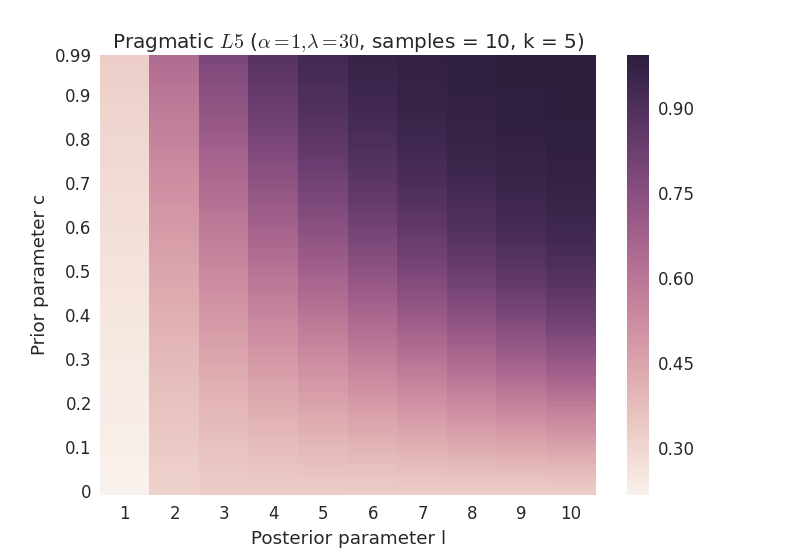
\includegraphics[scale=.5]{../presentations/01heatmap}
\caption{Mean proportion of pragmatic $L_5$ in $1000$ populations after $20$ generations ($\alpha = 1, \lambda = 30, k = 5$)}
\label{fig:prior-posterior}
\end{figure}



\subsection{Discussion}
Broadly speaking these results suggest that a lack of semantic upper-bounds coupled with pragmatic reasoning can overcome selective pressures and stabilize in a population provided there is a bias for simpler representations. This outcome is particularly encouraging in light of other advantages a lack of semantic upper-bounds may confer. 

This predictions hinges on three assumptions. First, that language is pressured toward both expressivity and learnability. Second, that language use is not too unpredictable: low $\alpha$ or $\lambda$ values renders languages that rely on pragmatics too prone to miscommunication and more difficult to learn. Third, that learners prefer simpler over more complex lexical representations. Importantly, a combination of rationality in learning and choice requires a weaker bias towards simpler representations. Under these conditions the selection of lexical meanings lacking upper-bounds in populations of pragmatic speakers is robust against parameter perturbations.

While a great representation of non upper-bounded lexical meanings is predicted by the literature, it is less clear to what extent other types should be represented -- if at all. There are reasons to expect functionally suboptimal types $L_1$-$L_3$ to be ruled out since they fail to enable their users to communicate effectively. However, this is not true of $L_4$.\footnote{$L_6$ presents a special case. In our current setup, it mirrors $L_5$ in enabling for a pragmatic strenghtening of message $m_2$ rather than $m_1$. However, this association of $s_2$ with $m_2$ under favourable parameter conditions is achieved by ruling out the ``some but not all''-state $s_1$ and not, as with scalar implicatures, the ``all''-state $s_2$. $L_6$ speakers therefore strenghten a ``some''-message to convey something paraphrasable as `some but not [some but not all]'. However, our present setup is blind to this redundancy.} Notwithstanding, it is possible that natural language communities are composed of homogeneous populations or that a single speaker may entertain $L_4$-like semantics for one scalar expression and $L_5$-like semantics for another.

This empirical issue relates to two aspects left undiscussed in our present analysis: disadvantages of pragmatic reasoning and the effect of state frequencies on the fossilization of pragmatic inferences. We tacitly assumed pragmatic reasoning to come at no cost. However, there is experimental evidence that suggests  that the pragmatic derivation of upper-bounds costs effort and takes additional processing time (cf. \citealt{deNeys+schaeken:2007, huang+snedeker:2009}. This raises the question at which point such usage-based cost undercuts the learnability advantage of simpler semantic representations. Should cost play a role, it's effect is bound to depend on the frequency with which a given scalar expression is used. We speculate that frequently drawn scalar implicatures might fossilize to avoid cost, while infrequent ones could still be computed on-line. 


\section{General discussion}
We laid out a model that combines game-theoretical models of functional pressure towards efficient communication \citep{nowak+krakauer:1999}, effects of learning biases on (iterated) language learning \citep{griffiths+kalish:2007}, probabilistic speaker and listener types of varied degrees of pragmatic sophistication \citep{frank+goodman:2012, franke+jaeger:2014} as well as different lexica \citep{bergen+etal:2012,bergen+etal:2016}. This model generates predictions about lexicalization patterns found in natural language. We argued that, while the puzzle raised by semantics in light of pragmatics is hard to explain on purely functional grounds, part of the answer lies in learnability: Simpler semantic representations are more likely to be learned while pragmatic reasoning can counteract functional disadvantages otherwise incurred. This result is of particular relevance for the longstanding assumption of a divide and interaction between semantics and pragmatics by offering an account of why (certain) pragmatic inferences are not part of the literal meaning of expressions.

%In sum, the innovation of this model lies in its combination of functional pressure on successful communication, effects of learning biases on (iterated) Bayesian language learning \citealt{griffiths+kalish:2007}, and probabilistic models of language use in populations with distinct lexica \citep{frank+goodman:2012,franke+jaeger:2014,bergen+etal:2016}. In particular, this synthesis enables for the investigation of the effects of communicative pressures on the semantics-pragmatics interface. In doing so, it links the previously disconnected areas of rational probabilistic language use and cultural evoltion.


\hl{Summarize main predictions: Only expressivity, only learnability, both together; expressivity nudging learning in the right direction and learning leading to a uniform preference for thing in the population}

Discussion about expressivity as external to learning (cf. Stadler, replicator-papers by Kenny Smith, Kirby et al 2015). Possibly add appendix with direct comparison between IL and RMD.

\hl{\citet{kirby+etal:2015} propose dynamics that involve expressivity and learnability. In contrast to our proposal, the former pressure is not fully decoupled from the latter in that is restricted to the production of learning data as a form of ambiguity avoidance (cf. brighton+etal:2005b cited on p.89l, who make render such ambiguity avoidance as a ``expressivity bias'' in learning). That is, a measure of the degree of understanding achieved by interlocutors is not a part of the theoretical model. }\footnote{\hl{We could say more about this}}

In contrast to past research using the replicator-mutator dynamics, the Bayesian setting afforded by iterated learning allows for a straightforward integration of a learning prior. Furthermore, less idiosyncratic assumptions about the variation introduced by learning without having to resort to similarity matrices between vocabularies \citep{nowak+krakauer:1999} nor languages \citep{nowak+etal:2002}.


Following \citet{piantadosi+etal:quantifiers} we assumed that, at some level, lexical meanings are expressed in a representational language and that the learners' task is to infer the lexicon that best explains the linguistic data they witness. We go beyond this by inferring type of use

\section{Conclusion}
Language change is affected by intertwined pressures. We investigated the selection of non-upper-bounded lexical meanings as a case study on role of semantics and pragmatics in satisfying such pressures. We showed that, when pressured for learnability and expressivity, the former drives for simpler semantic representations inasmuch as pragmatics can compensate for their lack of expressivity in use. That is, the relative learnability advantage of simpler semantics may offer an answer to why natural languages do not lexicalize certain pragmatic inferences. More broadly, we argued that semantic patterns can be explained by taking into consideration the way in which they are used in interactions as well as their representational complexity.


%%% Old snippets %%%
%\section{Conveying upper-bounds}
%Scalar inferences refer to the pragmatic derivation of an upper-bound for weak scalar expressions to the effect that stronger alternatives are inferred to not hold, e.g. {\em some students came} may be taken to convey that {\em not all students came}. The order of an expression such as {\em some} with respect to an alternative, e.g., {\em all}, is induced by entailment. For instance, {\em all students came} entails {\em most students came}, which in turn entails {\em some students came}. In this sense, {\em some} is weaker than {\em all}. A considerable class of natural language expressions do not lexicalize an upper-bound and can be ordered in this fashion, allowing for their pragmatic strengthening. As alluded at above, examples in English include numerals, scalar adjectives, quantifiers, modals, and connectives. \hl{possibly add some typological data on universality, frequency, monomorphemic status}
%
%The pragmatic enrichment of the semantic content of such expressions is enabled by mutual reasoning \citep{grice:1975}. More specifically, it is driven by interlocutors' mutual expectations of rational language use. The hearer reasons about the speaker's choice of a weak alternative over a stronger one. Had the speaker known that a stronger alternatives holds, she would have said so as this would have been more informative. Since she did not, the hearer can infer that the stronger alternative does not hold. Analogously, a speaker who reasons about her addressee may rely on her to derive this inference. In this way, a strengthened, upper-bounded, state of affairs can be conveyed without codifying the bound explicitly in the semantics.
%
%However, while pragmatics offers means to convey upper-bounds, the question why they are not part of the lexical meaning of these expressions remains. There are two main explanatory venues for this pattern. The first targets the functional advantages a lack of upper-bounds may confer to language users, whereas the second focuses on a learnability advantage of simpler over more complex semantic representations. 
%
%\paragraph{Function-based explanations.} Two assumptions are key to the pragmatic strengthening of weak alternatives: (the assumption of) cooperation and knowledge about the issue at hand. That is, the hearer needs to assume the speaker to be as informative as possible, i.e., not to withhold information, and that the speaker is knowlegeable, e.g., she knows whether {\em all students came}. Conversely, the speaker needs to assume the hearer to regard these conditions as satisfied. It is not difficult to imagine scenarios where either or both of these conditions are not given. For instance, the speaker may (be assumed to) not want to disclose all information about the students' attendance, or may have left early without being able to verify the attendance to a satisfactory degree. 
%
%\hl{Discussion of functional pressures for a lack of upper-bounds}

%\paragraph{Learning-based explanations.}
%
%\hl{Discussion of our main assumption that a lack of upper-bounds provides a learnability advantage framed in terms of relative representational simplicity over the codification of an upper-bound. {\bf Should this be made precise? If so, in which way?}}

%\bibliographystyle{apacite}
\bibliographystyle{unsrtnat}

%\setlength{\bibleftmargin}{.125in}
%\setlength{\bibindent}{-\bibleftmargin}
\bibliography{./bounds-rmd}


\end{document}
